\documentclass[11pt]{article}
\usepackage{tikz}
\usetikzlibrary{shadows,arrows,positioning}
% Define the layers to draw the diagram
\pgfdeclarelayer{background}
\pgfdeclarelayer{foreground}
\pgfsetlayers{background,main,foreground}
\pagenumbering{gobble}

% Define block styles
\tikzstyle{saberblock} = [draw, fill=orange!25, text centered, text width=5em, minimum height=4.2em, rounded corners, font=\bfseries]
\tikzstyle{fieldblock} = [draw, fill=blue!20, text centered, text width=5em, minimum height=4.2em, font=\bfseries]
\tikzstyle{arrow} = [draw, ultra thick, color=black!50, -latex']
\tikzstyle{line} = [draw, ultra thick, color=black!50]

% Define distances for bordering
\newcommand{\saberblock}[2]{node (s#1) [saberblock] {#2}}
\newcommand{\fieldblock}[2]{node (f#1) [fieldblock] {#2}}

\begin{document}
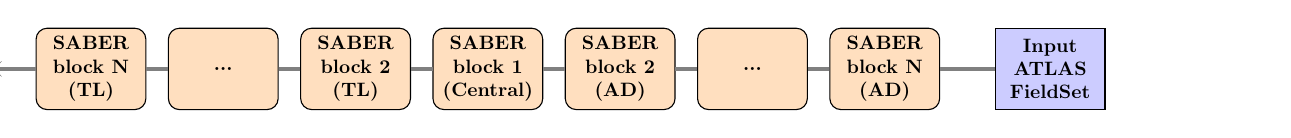
\begin{tikzpicture}[scale=0.7,transform shape]
\hspace{-2cm}
\path \fieldblock{1}{Output\\ATLAS\\FieldSet};
\path (f1)+(3.0,0.0) \saberblock{1}{SABER\\block N\\(TL)};
\path (s1)+(2.4,0.0) \saberblock{2}{...};
\path (s2)+(2.4,0.0) \saberblock{3}{SABER\\block 2\\(TL)};
\path (s3)+(2.4,0.0) \saberblock{4}{SABER\\block 1\\(Central)};
\path (s4)+(2.4,0.0) \saberblock{6}{SABER\\block 2\\(AD)};
\path (s6)+(2.4,0.0) \saberblock{7}{...};
\path (s7)+(2.4,0.0) \saberblock{8}{SABER\\block N\\(AD)};
\path (s8)+(3.0,0.0) \fieldblock{2}{Input\\ATLAS\\FieldSet};

\path [arrow] (s1.west) -- (f1.east) node[] {};
\path [line] (s2.west) -- (s1.east) node[] {};
\path [line] (s3.west) -- (s2.east) node[] {};
\path [line] (s4.west) -- (s3.east) node[] {};
\path [line] (s6.west) -- (s4.east) node[] {};
\path [line] (s7.west) -- (s6.east) node[] {};
\path [line] (s8.west) -- (s7.east) node[] {};
\path [line] (f2.west) -- (s8.east) node[] {};
\end{tikzpicture}

\end{document}
